\section{Introduction}
\label{sec:intro}

Unifying visual understanding and generation within the pure autoregressive (AR) paradigm of Large Language Models (LLMs) offers a simple, end-to-end alternative to the increasingly common yet structurally complex approach of coupling LLMs with external diffusion modules~\citep{dong2024dreamllm,huang2025illume+,metaquery,blip3o}. To enable fully unified AR modeling of vision and language, a model requires a visual tokenizer to map images into discrete tokens and a corresponding detokenizer that can faithfully reconstruct them back into pixel space.


% \begin{figure}[t]
%   \centering
  
%   \begin{minipage}[t]{0.504\textwidth}
%   \centering
%   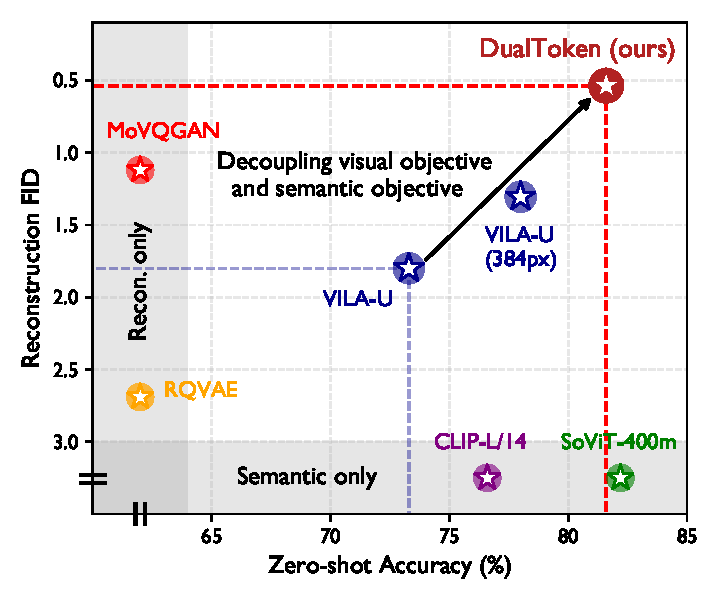
\includegraphics[height=5.2cm]{imgs/bubble.pdf}
%   \end{minipage}
%   \begin{minipage}[t]{0.44\textwidth}
%   \centering
%   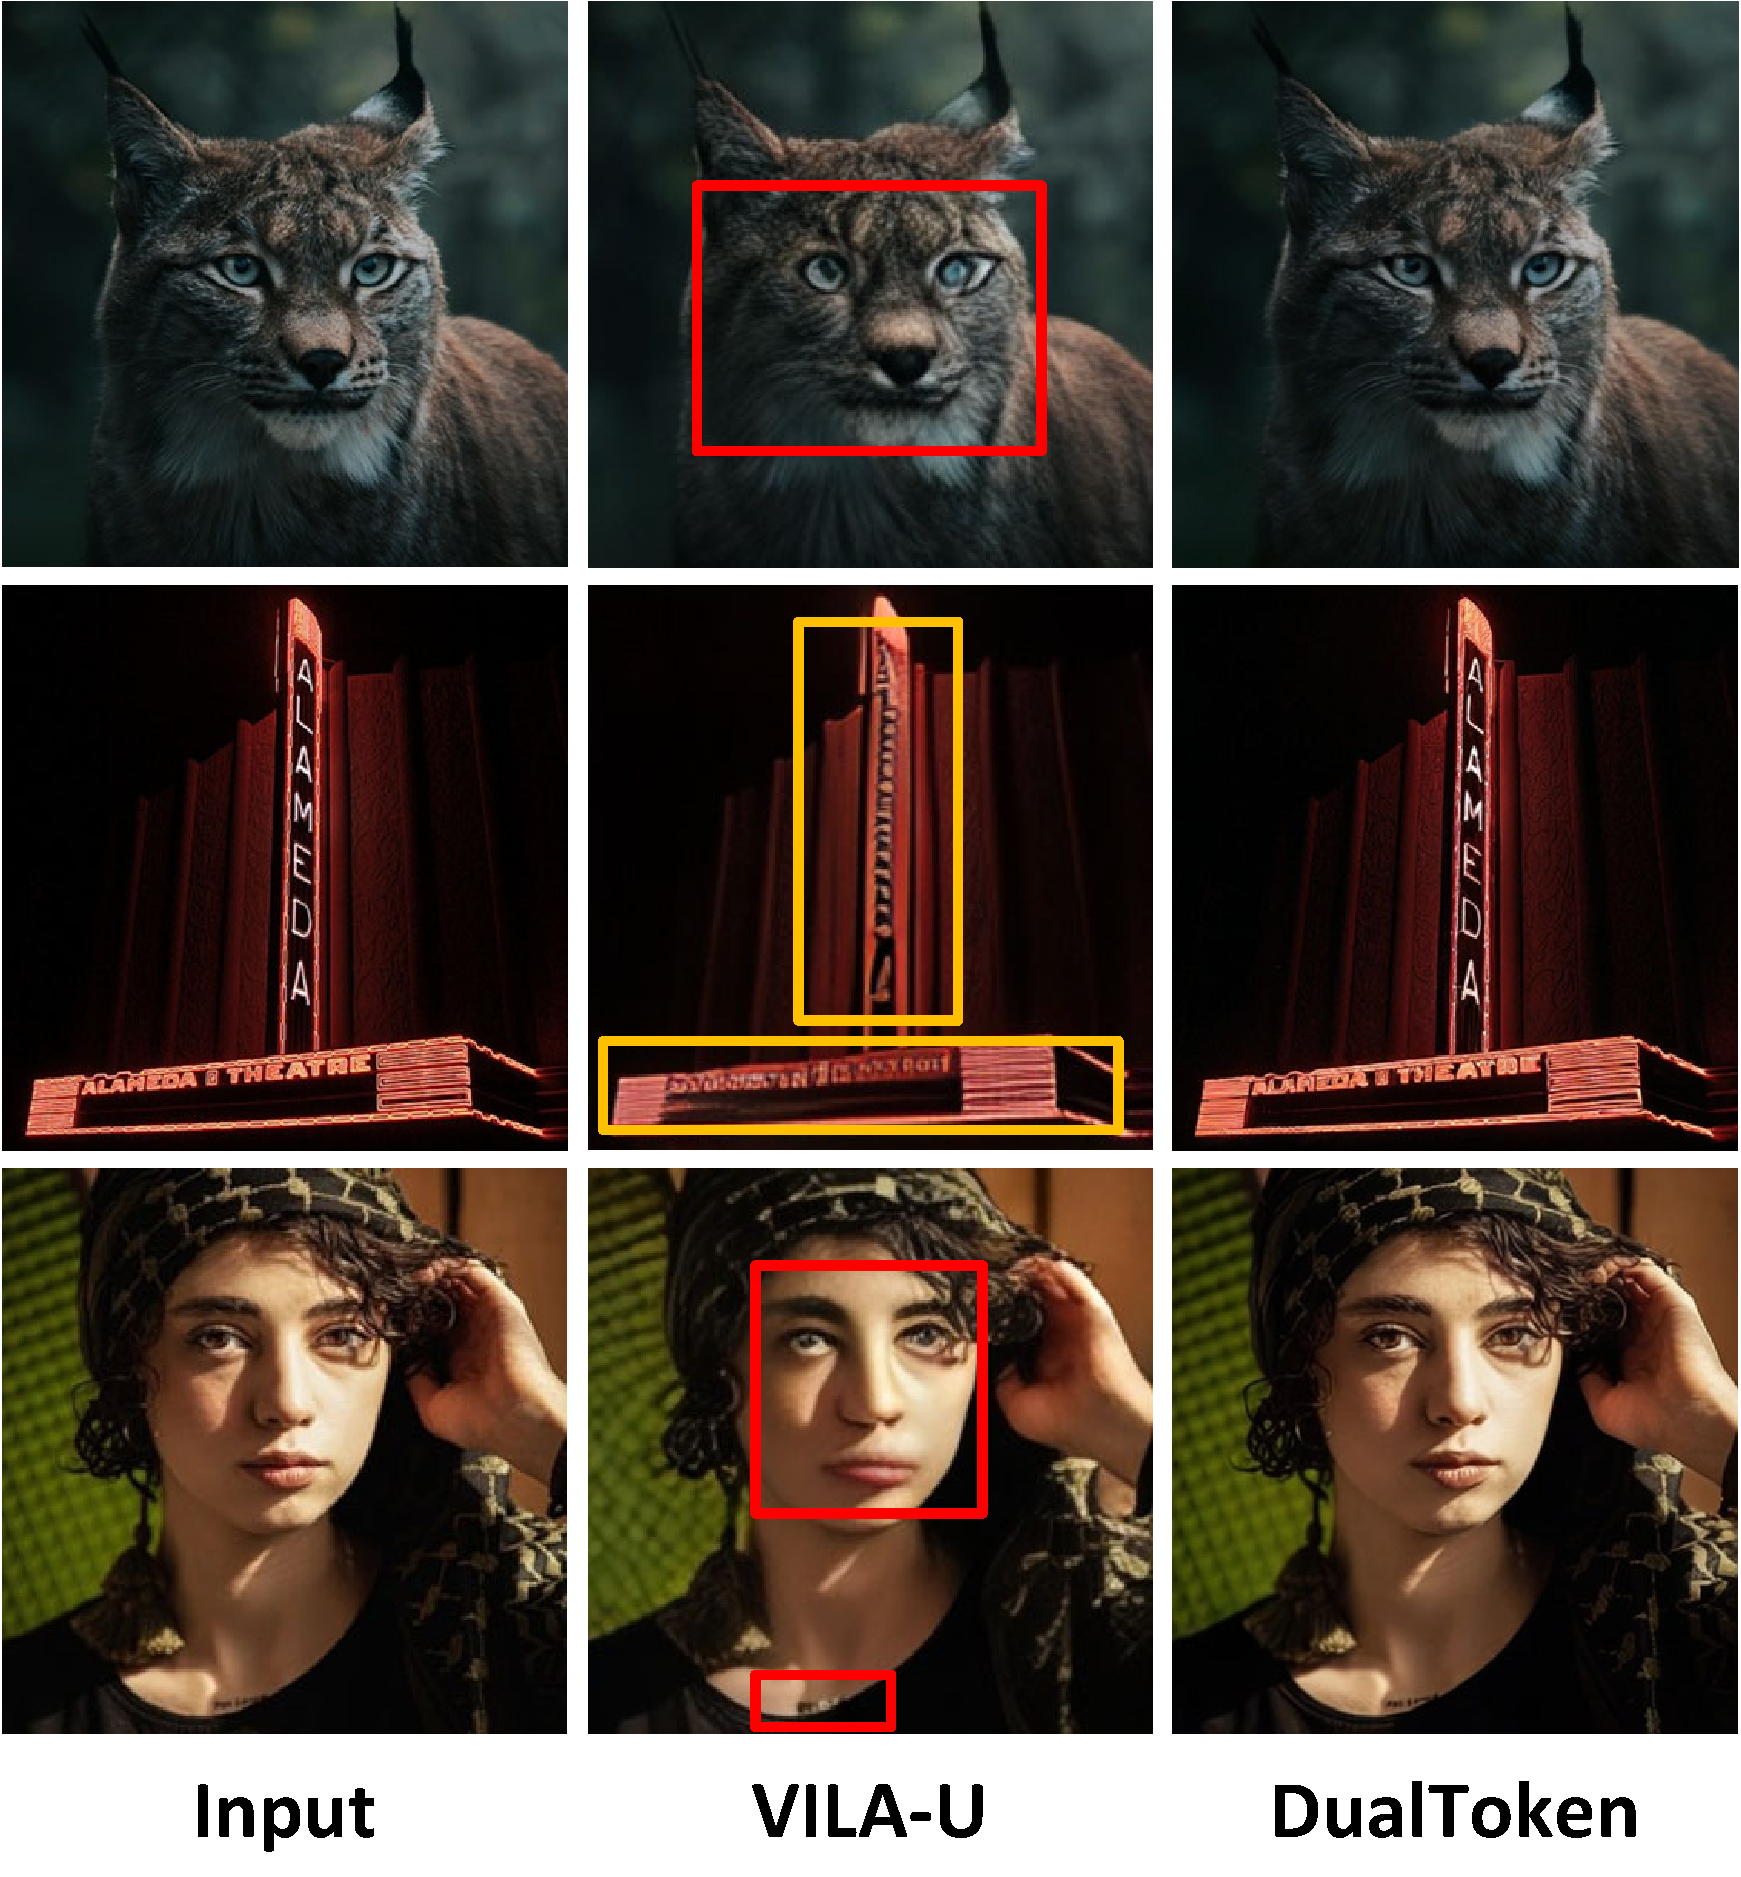
\includegraphics[height=5.2cm]{imgs/teaser.pdf}
%   \end{minipage}
%   \caption{
%     \textbf{Comparison with state-of-the-art vision encoders.} \textbf{(Left)} We compare zero-shot classification accuracy and reconstruction FID on ImageNet-1K(val) across baseline methods and \ours{}. \ours{} achieves results comparable to or surpassing both semantic-only and reconstruction-only methods in both tasks. \textbf{(Right)} Reconstruction results of VILA-U and \ours{}, our \ours{} significantly outperforms VILA-U, which suffers from severe distortion and blurriness.
%   }
%   \label{fig:Bubble}
% \end{figure}

\begin{figure}[ht]
  \centering
  \vspace{-0.2cm}
  \begin{minipage}[t]{0.435\textwidth}
  \centering
  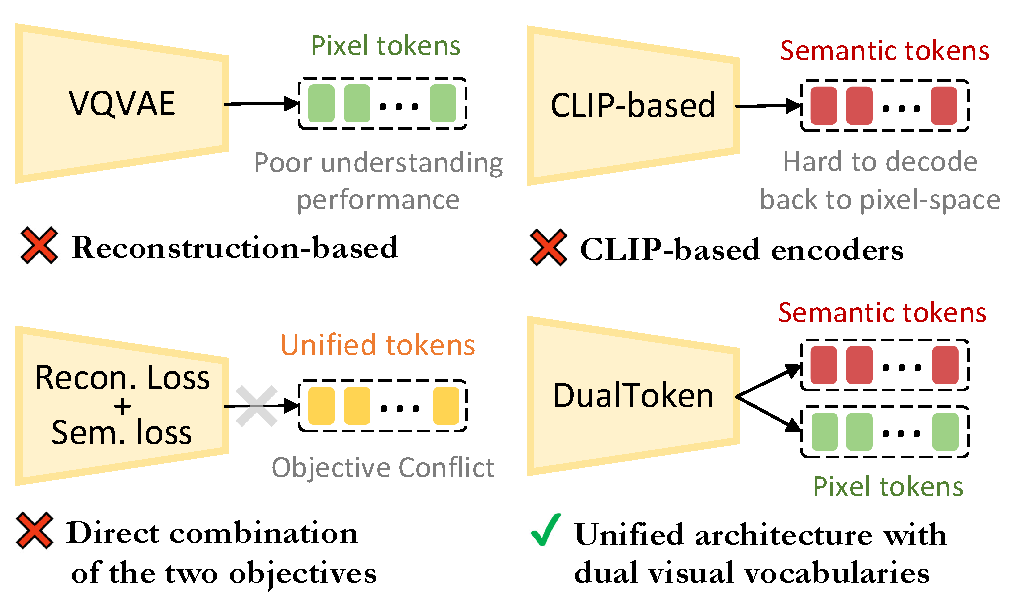
\includegraphics[height=3.5cm]{imgs/teaser_framework-v6.pdf}
  \end{minipage}
  \begin{minipage}[t]{0.303\textwidth}
  \centering
  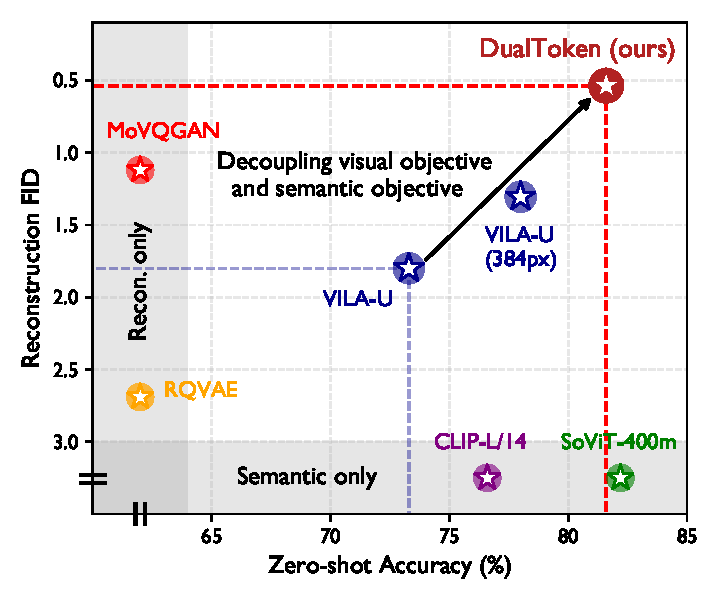
\includegraphics[height=3.5cm]{imgs/bubble.pdf}
  \end{minipage}
  \begin{minipage}[t]{0.250\textwidth}
  \centering
  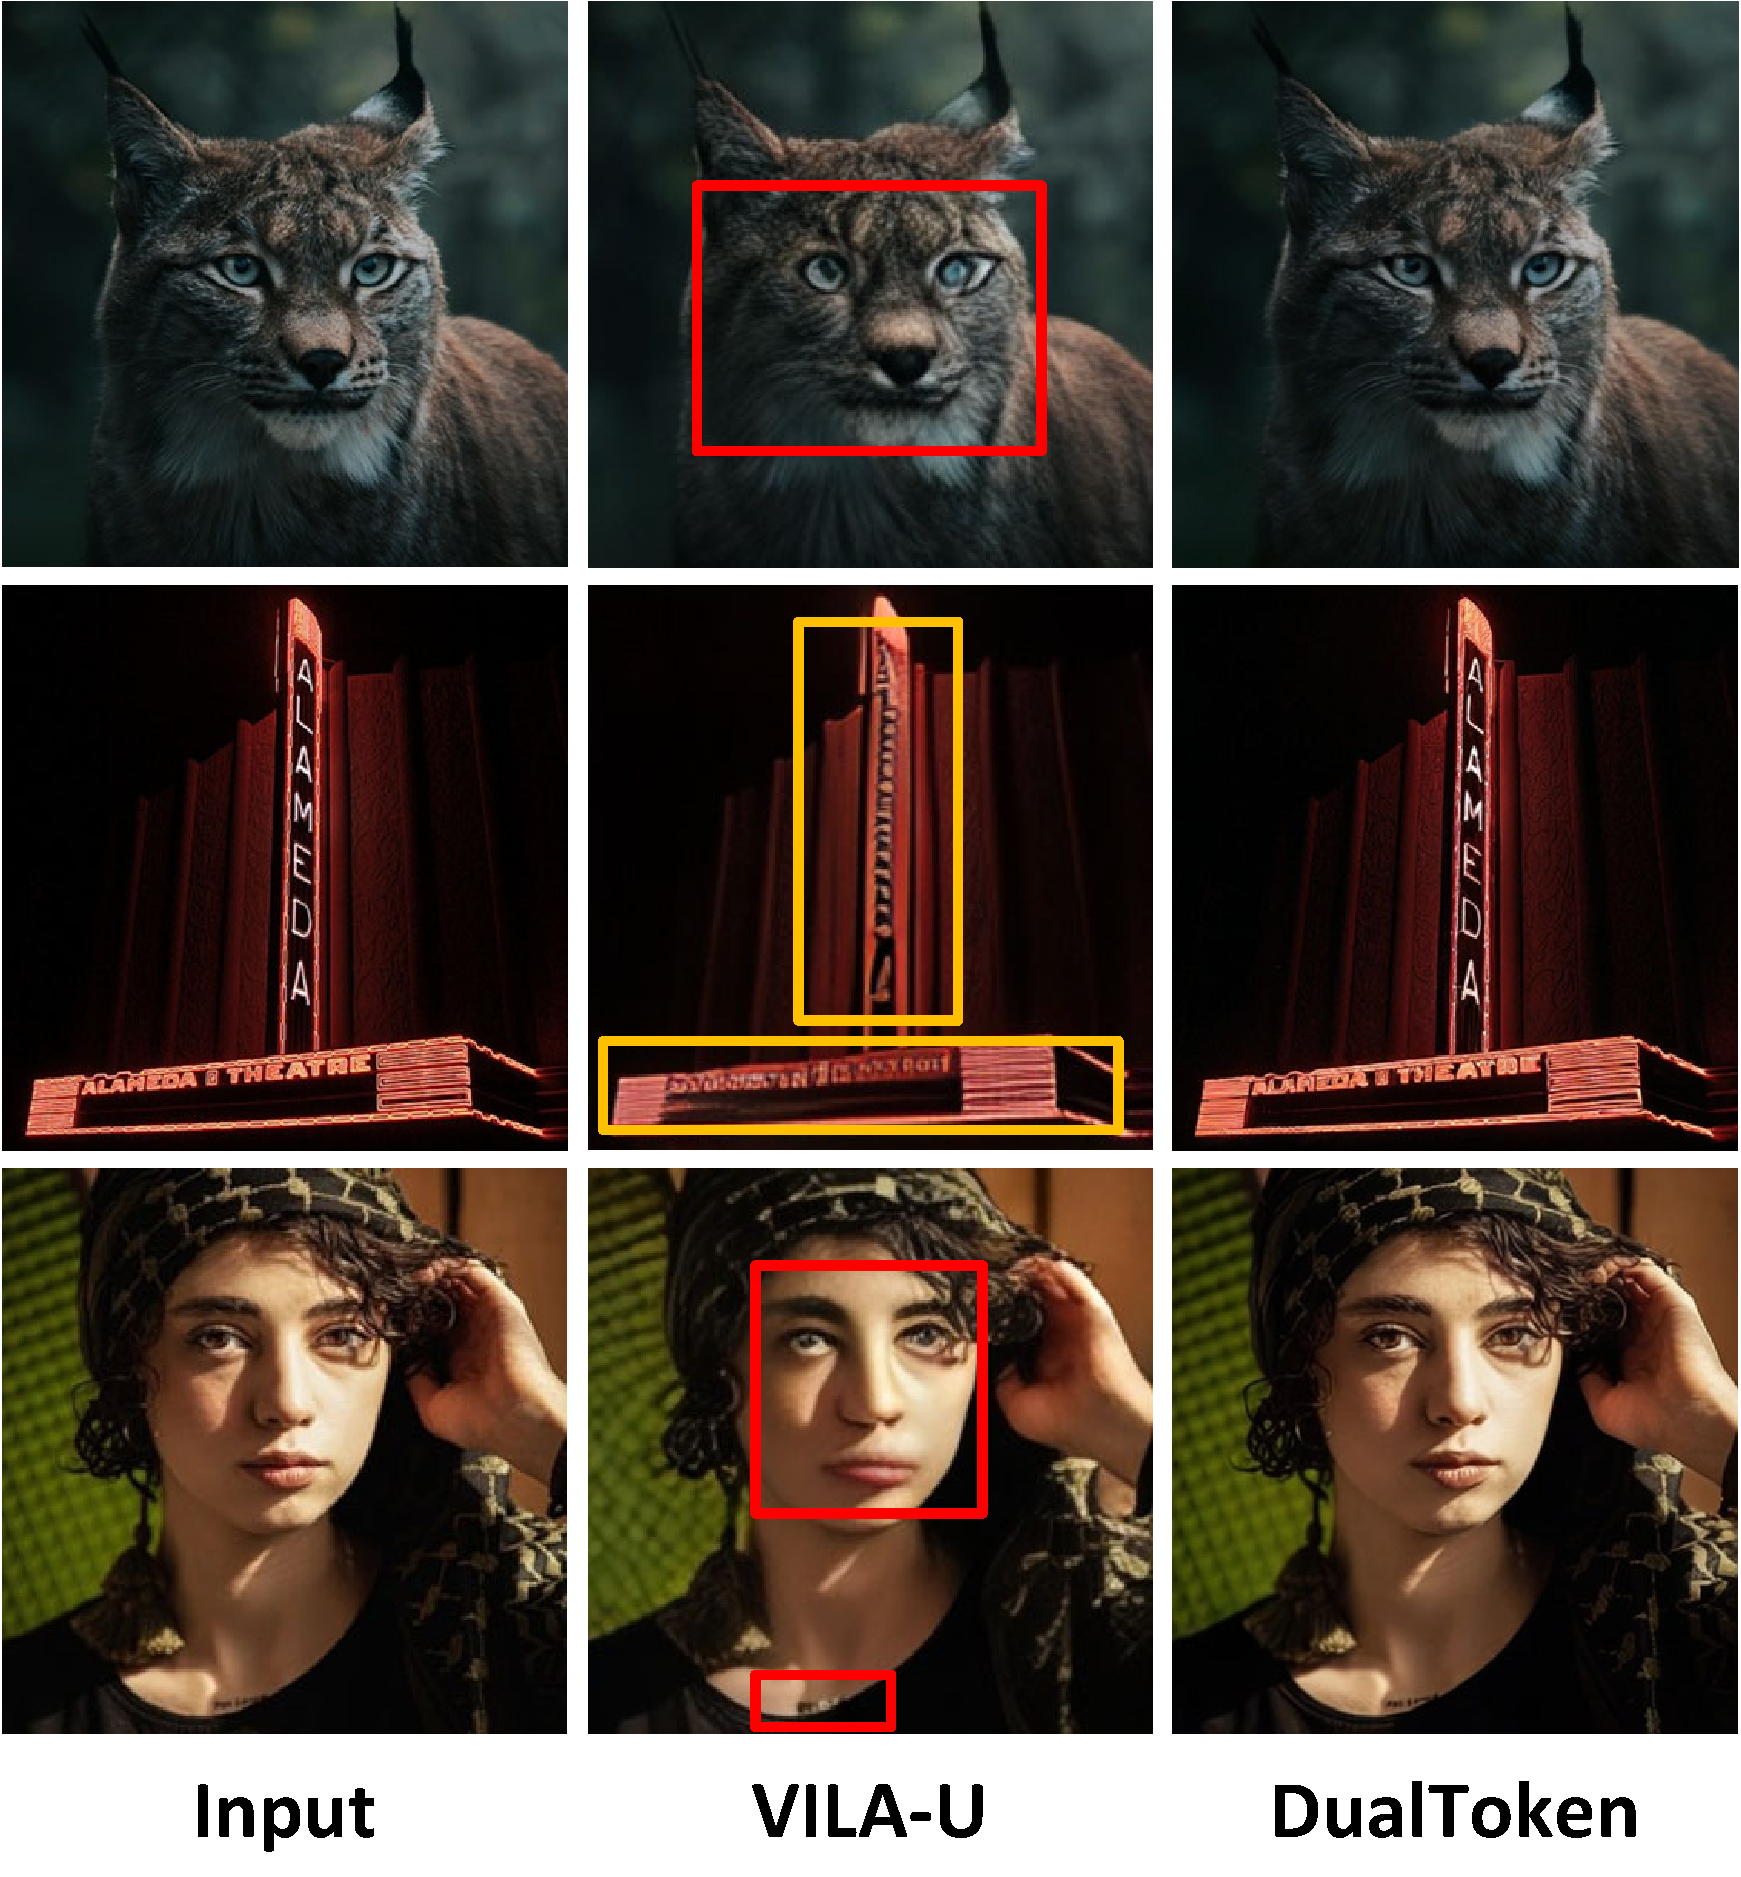
\includegraphics[height=3.5cm]{imgs/teaser.pdf}
  \end{minipage}
  
  \caption{
    \textbf{(Left)} Challenges faced by existing visual tokenizers. \textbf{(Middle)} We compare zero-shot classification accuracy and reconstruction FID on ImageNet-1K(val) across baseline methods and \ours{}. \ours{} achieves results comparable to or surpassing both semantic-only and reconstruction-only methods in both tasks. \textbf{(Right)} Reconstruction results of VILA-U and \ours{}, our \ours{} significantly outperforms VILA-U, which suffers from severe distortion and blurriness.
  }
  \label{fig:Bubble}
  % \vspace{-10pt}
  \vspace{-0.45cm}
\end{figure}


Early methods in this direction~\citep{yu2023CM3leon,team2024chameleon,wang2024emu3} directly adopt the encoder and decoder of VQ-VAE as the visual tokenizer and detokenizer. While these approaches demonstrated the feasibility of unifying visual understanding and generation within the AR paradigm, their understanding capabilities are typically lacking compared to multimodal large language models (MLLMs) specialized for understanding tasks~\citep{liu2023mmbench,yue2023mmmu,fu2024mme,song2024m3gia}.
We argue that this performance gap stems from inadequate visual representations: traditional VQ-VAEs are optimized solely for reconstruction, producing image tokens that preserve low-level visual details but fail to capture high-level semantics aligned with language. By contrast, MLLMs designed for understanding tasks~\citep{liu2024llavanext,chen2024sharegpt4v,li2024baichuanomni,li2025baichuanomni1d5,qwen2d5vl} typically rely on CLIP-family encoders~\citep{radford2021clip,zhai2023siglip}, which are pretrained with text alignment and thus inherently encode high-level semantics, making them more suitable for downstream visual understanding tasks in MLLMs.

\begin{minipage}[t]{0.44\textwidth}
    To fully leverage the language-aligned semantic representations of CLIP, a natural approach is to quantize the features of a CLIP encoder and train a decoder for image reconstruction~\citep{wu2025vilau}. This involves learning to reconstruct images for downstream generation tasks while preserving its semantic capabilities as much as possible~\citep{wu2025vilau}.
    However, as shown in Fig.\ref{fig:Bubble} and Table.\ref{tab:tokenizers}, directly combining reconstruction and semantic objectives often leads to severe distortions and blurriness in reconstruction tasks, along with a noticeable decline in semantic metrics such as zero-shot classification and image-text retrieval, compared to its original pretrained model \citep{zhai2023siglip}.
    This degradation, as discussed in \citet{wu2025vilau}, reflects the inherently conflict between the two training objectives, ultimately limiting both the quality of downstream image generation tasks and the performance of multimodal understanding tasks.
\end{minipage}
\hfill
\begin{minipage}[t]{0.545\textwidth}
\vspace{-0.25cm}
    \centering
    \captionsetup{type=table}
    \caption{
        \textbf{Comparison to state-of-the-art visual tokenizers.} DualToken achieves the best performance among existing unified visual tokenizers in semantic metrics. It also mitigates the distortion and blurriness faced by VILA-U during reconstruction, and surpasses dedicated models in reconstruction metrics.
    }
    \vspace{-0.225cm}
    \label{tab:tokenizers}
    \tablestyle{2pt}{1.108}
    \resizebox{0.97\linewidth}{!}{
    \begin{tabular}{lcccccc}
    \toprule
     \multirow{2}{*}{\textsc{Methods}} & \multicolumn{3}{c}{Semantic}&\multicolumn{3}{c}{Reconstruction}\\ 
     \cmidrule{2-7}&     Zero-Shot\higherbetter & T2I(R@1)\higherbetter &I2T(R@1)\higherbetter &rFID\lowerbetter  &PSNR\higherbetter  &SSIM\higherbetter \\
    \midrule
     \multicolumn{7}{l}{\textbf{\textit{Reconstruction Only}}}\\
     % VQGAN~\citep{esser2021vqgan}                           &\textcolor{red}{\ding{55}}  &\textcolor{red}{\ding{55}}         &\textcolor{red}{\ding{55}}  &4.98   & -      &-\\
     MoVQGAN~\citep{zheng2022movq}                          &\textcolor{red}{\ding{55}}  &\textcolor{red}{\ding{55}}         &\textcolor{red}{\ding{55}}  &1.12   &22.42   &0.673\\
     RQ-VAE~\citep{lee2022rqvae}                            &\textcolor{red}{\ding{55}}  &\textcolor{red}{\ding{55}}         &\textcolor{red}{\ding{55}}  &2.69   &-       &-\\
     ViT-VQGAN~\citep{yu2021vitvqgan}                       &\textcolor{red}{\ding{55}}  &\textcolor{red}{\ding{55}}         &\textcolor{red}{\ding{55}}  &1.55   &-       &-\\
     Open-MAGVIT2~\citep{luo2024openmagvit2}                &\textcolor{red}{\ding{55}}  &\textcolor{red}{\ding{55}}         &\textcolor{red}{\ding{55}}  &1.17   &21.90   &-\\
     SBER-MoVQGAN~\citep{sber2023movqgan}                   &\textcolor{red}{\ding{55}}  &\textcolor{red}{\ding{55}}         &\textcolor{red}{\ding{55}}  &{0.68} &{27.04} &{0.741}\\
     % FQGAN-Dual ($\downarrow$16)~\citep{bai2024fqgan}     &\textcolor{red}{\ding{55}}  &\textcolor{red}{\ding{55}}         &\textcolor{red}{\ding{55}}  &0.94   &22.02   &-\\
     % FQGAN-Triple ($\downarrow$16)~\citep{bai2024fqgan}   &\textcolor{red}{\ding{55}}  &\textcolor{red}{\ding{55}}         &\textcolor{red}{\ding{55}}  &0.76   &22.73   &-\\
     \midrule
     \multicolumn{7}{l}{\textbf{\textit{Understanding Only}}}\\
     CLIP-L/14-336~\citep{radford2021clip}             &{76.6}            &{21.2}    &{21.5}   &\textcolor{red}{\ding{55}}  &\textcolor{red}{\ding{55}}  &\textcolor{red}{\ding{55}} \\
     SigLIP-L/16-256~\citep{zhai2023siglip}            &{80.5}            &{21.0}    &{21.4}   &\textcolor{red}{\ding{55}}  &\textcolor{red}{\ding{55}}  &\textcolor{red}{\ding{55}} \\
     SigLIP-So/14-384~\citep{zhai2023siglip}           &{83.2}            &{21.7}    &{21.6}   &\textcolor{red}{\ding{55}}  &\textcolor{red}{\ding{55}}  &\textcolor{red}{\ding{55}} \\
     SigLIP2-So/16-256~\citep{tschannen2025siglip2}    &{83.4}            &{21.5}    &{22.0}   &\textcolor{red}{\ding{55}}  &\textcolor{red}{\ding{55}}  &\textcolor{red}{\ding{55}} \\
     ViTamin-L/16-256~\citep{chen2024vitamin}          &{81.2}            &{20.6}    &{21.2}   &\textcolor{red}{\ding{55}}  &\textcolor{red}{\ding{55}}  &\textcolor{red}{\ding{55}} \\
     \midrule
     \multicolumn{7}{l}{\textbf{\textit{Reconstruction \& Understanding}}}\\
     % SeTok~\citep{SeTok}                               &75.4              &-         &-        &2.07           &-                &-\\
     QLIP ($256px$)~\citep{zhao2025qlip}               &74.3              &16.8      &18.4     &3.21           &23.16            &0.628\\
     QLIP ($392px$)~\citep{zhao2025qlip}               &79.1              &20.4      &21.0     &1.46           &25.36            &0.690\\
     UniTok~\citep{unitok}                             &78.6              &-         &-        &0.38           &25.34            &-\\
     TokenFlow ($256px$)~\citep{qu2024tokenflow}       &-                 &-         &-        &1.37           &21.41            &0.687\\
     TokenFlow ($384px$)~\citep{qu2024tokenflow}       &-                 &-         &-        &0.63           &22.77            &0.731\\
     Muse-VL ($256px$)~\citep{xie2025musevl}           &-                 &-         &-        &2.26           &20.14            &0.646\\
     TokLIP (SigLIP2-So/16-384)~\citep{lin2025toklip}            &80.0              &-         &-        &0.94           &21.94            &0.726\\
     VILA-U (SigLIP-L/16-256)~\citep{wu2025vilau}      &73.3              &10.0      &11.2     &1.80           &3.43             &0.489\\
     VILA-U (SigLIP-So/14-384)~\citep{wu2025vilau}     &78.0              &-         &-        &1.25           &-                &-\\
     \compare{}\ours{} (SigLIP-L/16-256)               &\compare{}{79.8}  &\compare{}{20.8} &\compare{}{21.4} &\compare{}{1.06} &\compare{}{27.12} &\compare{}{0.693} \\
     \compare{}\ours{} (SigLIP-So/14-384)              &\compare{}{82.0}  &\compare{}{21.5} &\compare{}{21.6} &\compare{}{0.25} &\compare{}{28.69} &\compare{}{0.744}\\
     \compare{}\ours{} (SigLIP2-So/16-256)             &\compare{}{82.3}  &\compare{}{21.1} &\compare{}{21.9} &\compare{}{0.52} &\compare{}{28.03} &\compare{}{0.726} \\
    \bottomrule
    \end{tabular}}
\end{minipage}

To disentangle the two conflicting objectives, we propose \emph{interpreting visual appearance and visual semantics---required for visual generation and understanding---as distinct visual vocabularies}: a pixel codebook that captures low-level appearance features for generation, and a semantic codebook that encodes high-level semantic features essential for understanding.
Specifically, inspired by the hierarchical structure of the human visual system \citep{groen2017contributions}, we partition the Vision Transformer (ViT)~\citep{dosovitskiy2020ViT} into shallow, middle, and deep stages based on the cosine similarity \citep{chen2025rethinking} across layers and observe that shallow layers of a ViT predominantly capture low-level perceptual information—such as texture and color—making them suitable for reconstruction tasks, whereas high-level semantic representations emerge in the deeper layers \citep{chen2023building,chen2025rethinking}.
To fully exploit this inherent property of ViT, we utilize shallow-layer features for reconstruction and deep-layer features for semantic learning, thereby enabling the simultaneous derivation of both a pixel codebook and a semantic codebook within a unified tokenizer.

% Surprisingly, this hierarchical decoupling not only resolves the conflict between the two objectives but also enables the semantic learning objective to enhance low-level reconstruction. Moreover, training the shallow-layer reconstruction task introduces minimal degradation to the model’s original semantic capabilities, without additional contrastive learning stages~\citep{radford2021clip,wu2025vilau}. As a result, our DualToken achieves the best semantic performance among established unified tokenizers~\citep{wu2025vilau,zhao2025qlip,qu2024tokenflow,unitok} while also attaining state-of-the-art performance in reconstruction.
This hierarchical decoupling effectively resolves the conflict between the two objectives. 
% On the one hand, it mitigates the semantic learning objective to enhance low-level reconstruction. Moreover, training the shallow-layer reconstruction task introduces minimal degradation to the model’s original semantic capabilities, without additional contrastive learning stages~\citep{radford2021clip,wu2025vilau}. 
As a result, our DualToken achieves the best semantic performance among established unified tokenizers~\citep{wu2025vilau,zhao2025qlip,qu2024tokenflow,unitok} while also attaining state-of-the-art performance in reconstruction.
Building upon this, we further demonstrate how a MLLM can effectively utilize the dual visual vocabularies to achieve unified vision understanding and generation.

Our analysis reveals three key findings:
i) \textbf{Dual visual vocabularies resolve conflicts}: Decoupling visual appearance and visual semantics with separate visual vocabularies mitigates the conflict between reconstruction and semantic objectives.
% and transform them into a positive relationship.
Our tokenizer achieves state-of-the-art performance in both sides, using only 10\% of the pretraining data required by VILA-U;
ii) \textbf{DualToken is better than combining dual encoders}: We observe that DualToken, as a unified architecture, outperforms the direct combination of two heterogeneous visual encoders, demonstrating both simplicity and effectiveness;
iii) \textbf{Dual-token promote each other}: On one hand, visual appearance tokens (pixel tokens) are not only used for generation but also contribute fine-grained low-level features that enhance visual understanding. On the other hand, visual semantic tokens---beyond their role in understanding tasks---act as positive supervision during autoregressive generation, leading to more semantically aligned image outputs compared to generating pixel tokens alone.